
%(BEGIN_QUESTION)
% Copyright 2011, Tony R. Kuphaldt, released under the Creative Commons Attribution License (v 1.0)
% This means you may do almost anything with this work of mine, so long as you give me proper credit

These two control valves are split-ranged, driven by a common pneumatic output signal from one I/P transducer.  The bench set range for each valve is specified as necessary to create the split-range sequencing:

$$\includegraphics[width=15.5cm]{i01989x01.eps}$$

Calculate each valve position (in percentage open: 0\% being fully shut and 100\% being fully open), assuming a current signal to the I/P of 15.6 mA:

\vskip 20pt

\hskip 50pt PV-33a = \underbar{\hskip 50pt} \% open \hskip 60pt PV-33b = \underbar{\hskip 50pt} \% open

\underbar{file i01989}
%(END_QUESTION)





%(BEGIN_ANSWER)

PV-33a = \underbar{\bf 45} \% open \hskip 100pt PV-33b = \underbar{\bf 0} \% open

%(END_ANSWER)





%(BEGIN_NOTES)

{\bf This question is intended for exams only and not worksheets!}.

%(END_NOTES)

